\section{Results}

\subsection{Signal outputs}
The output wave-forms as seen on the oscilloscope for different values of loads and capacitance are shown here in Figs. 5 to 8.

\begin{figure}[H]
    \centering
    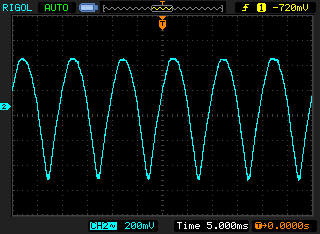
\includegraphics[width=0.67\columnwidth]{images/03.png}
    \caption{Full wave rectifier signal output  without a filter at $R = 9.86\,k\Omega$ ($r=0.533$)}
\end{figure}

\begin{figure}[H]
    \centering
    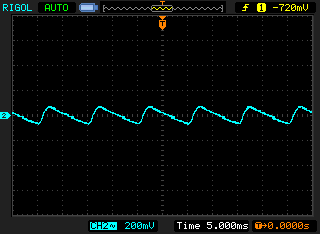
\includegraphics[width=0.67\columnwidth]{images/11.png}
    \caption{Full wave rectifier signal output with a filter at $R = 2.167\,k\Omega$ and $C = 23.05\,\mu F$ ($r=0.050$)}
\end{figure}

\begin{figure}[H]
    \centering
    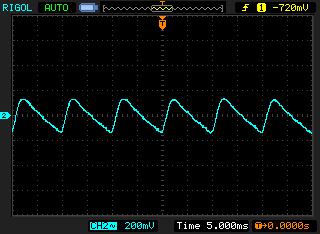
\includegraphics[width=0.67\columnwidth]{images/21.png}
    \caption{Half wave rectifier signal output with a filter at $R = 2.167\,k\Omega$ and $C = 10.4\,\mu F$ ($r=0.103$)}
\end{figure}

\begin{figure}[H]

     \centering
     \begin{subfigure}{1\columnwidth}
        \centering
        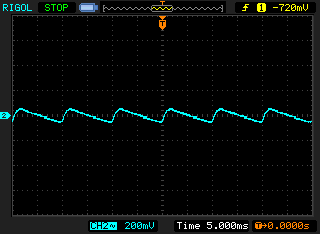
\includegraphics[width=0.67\columnwidth]{images/31.png}
        \caption{$R =2.167\,k\Omega$ ($r=0.036$)}
    \end{subfigure}
    
    \begin{subfigure}{1\columnwidth}
        \centering
        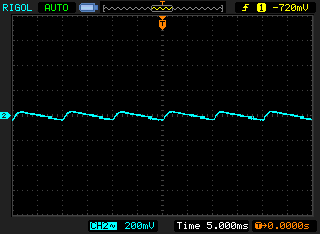
\includegraphics[width=0.67\columnwidth]{images/32.png}
        \caption{$R =3.846\,k\Omega$ ($r=0.021$)}
    \end{subfigure}

    \begin{subfigure}{1\columnwidth}
        \centering
        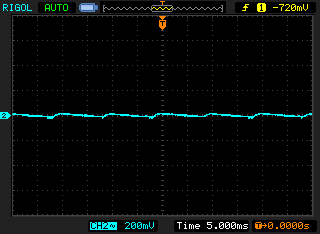
\includegraphics[width=0.67\columnwidth]{images/33.png}
        \caption{$R =9.862\,k\Omega$ ($r=0.008$)}
    \end{subfigure}
    
    \caption{Full wave rectifier signal output for a particular $C = 37.47\,\mu F$, for increasing values of $R$. Notice how the ripple in the signal decreases. The signal for the circuit with maximum measured values of $RC$ is very close to a straight line.}
\end{figure}

\subsection{Error Analysis}
For the full-wave rectifier circuit without a filter, we can measure the error in $r$ as,

\begin{equation*}
    \frac{\Delta r}{r} = \sqrt{\left(\frac{\Delta V_{ac}}{V_{ac}}\right)^2 + \left(\frac{\Delta V_{dc}}{V_{dc}}\right)^2}
\end{equation*}

where $\Delta V_{ac}$ and $\Delta V_{dc}$ are the least count of the voltmeters. And the average error can be found by,

\begin{equation*}
    \Delta r = \frac{1}{3}\sqrt{(\Delta r_1)^2 + (\Delta r_2)^2 + (\Delta r_3)^2}.
\end{equation*}

Thus, the calculated value of $\Delta r = 0.001$. 

Similarly, rectification efficiency can be calculated as,

\begin{equation*}
    \eta = \frac{V_{dc}^2/R_L}{I_{ac}V_{ac(\text{input})}}
\end{equation*}

Therefore the error in rectification efficiency would be,

\begin{equation*}
    \frac{\Delta \eta}{\eta} = \sqrt{\left(\frac{\Delta V_{ac}}{V_{ac}}\right)^2 + \left(\frac{2\Delta V_{dc}}{V_{dc}}\right)^2 + \left(\frac{\Delta I_{ac}}{I_{ac}}\right)^2 + \left(\frac{\Delta R_{L}}{R_{L}}\right)^2}
\end{equation*}

where $\Delta R_L$ and $\Delta I_{ac}$ are the least count of the multi-meter readings. The average value of $\Delta \eta$ can be calculated similar to that of $\Delta r$, which comes out to be $\Delta \eta = 0.11\%$. 

\section{Conclusion}
For the full-wave rectifier circuit without the filter, we can see that the ripple factor and rectification efficiency stays around the same for different loads with an average value,

\begin{align*}
    r &= 0.539 \pm 0.001\\
    \eta &= (66.82 \pm 0.11)\%
\end{align*}

where $r$ is close to the theoretically calculated value and the rectification efficiency is less than the ideal value, as predictable.

For the full-wave rectifier circuit with the filter, we can see that for a particular capacitance, $r$ is inversely proportional to the load resistance. Similarly, for a particular load resistance, $r$ is inversely proportional to capacitance. For the highest given values of $RC$, $r = 0.008$ (Fig. 8(c)). 

Since we are ideally aiming for the lowest ripple factor in the output signal (i.e. maximise the DC component), we can conclude that a proper combination of optimally large values of RC will give us a steady output signal.

\section{Precautions}
\begin{enumerate}
    \item The transformer must be handled carefully.
    \item Switch on the circuit only after verifying the connections to be proper.
    \item Visualise the output on the oscilloscope to make sure the rectification is happening before taking readings.
    \item Do not change the resistor or the capacitor while the circuit is switched on.
\end{enumerate}